%Correct the file name.
%X: book number
%Y: part number
%ZZZ: page number in three digits. So page 3 would be 003.

\documentclass[9pt]{amsbook}

\usepackage{../HBSuerDemir}	% ------------------------
\usepackage{wrapfig}
\usepackage{setspace}
\usepackage{float}
\begin{document}

% ++++++++++++++++++++++++++++++++++++++
\hPage{b1p2/501}
% ++++++++++++++++++++++++++++++++++++++
\newtheorem{theorem}{Theorem}
\setcounter{section}{8}
\setcounter{page}{501}

% =======================================
roid of the generating arc (region). They are extremely useful
for finding the centroid when surface area (volume) is known,
and for finding the latter when the centroid is known. \\
% -------------------------------------------------------------------
\begin{wrapfigure}{r}{5.5cm}
	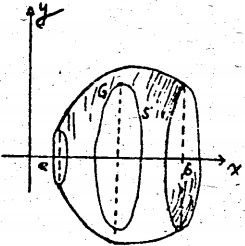
\includegraphics{images/b1p2-501-fig01.png}
\end{wrapfigure}
% -------------------------------------------------------------------
\begin{thm}
		The area of a surface of revolution generated
	by revolving an arc about a line in its plane not cutting the
	arc, is equal to the product of the length of arc and the circumference
	of the circle described by the centroid of the arc: \\
		$S_{0x} = s . 2 \pi \overline{y}$ .

\end{thm}
% -------------------------------------------------------------------
\begin{proof}
\begin{flushleft}
	{\setstretch{1.5}
		Let the arc of the curve \\
		$ y = f(x)\in D\big(a, b\big) , \qquad y\geq0$ \\
		be revolved about the x-axis. We have \\
		$S_{0x} = 2\pi \int_{a}^{b} y ds$ \\
		as the area of the surface, and \\
		$s \overline{y} = M_{0x} = \int_{a}^{b} y ds \qquad (\delta = 1)$ \\
		$S_{0x} = 2\pi . s\overline{y} = s . 2\pi \overline{y}$ \\
	}
\end{flushleft}
\end{proof}

% -------------------------------------------------------------------
\begin{thm}
		The volume of a solid of revolution generated
	by revolving a region about a line in its plane not cutting the 
	region, is equal to the product of the area of the region and 
	the circumference of the circle described by the centroid of 
	the region.
\end{thm}
% -------------------------------------------------------------------
\begin{wrapfigure}{r}{5.5cm}
	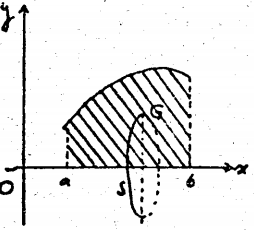
\includegraphics{images/b1p2-501-fig02.png}
\end{wrapfigure}
% -------------------------------------------------------------------
\begin{proof}
\begin{flushleft}
	{\setstretch{1.5}
		Let the region be \\
		$ R_{xy} = \Bigg(a, b;\ y_1(x),\ y_2(x)\Bigg)$  \\
		be revolved about the x-axis. We have \\
		$V_{0x} = \pi \int_{a}^{b} (y_2^2-y_1^2) dx$ \\
		as the volume of the solid, and \\
	}
\end{flushleft}
\end{proof}
% =======================================




% =======================================




% =======================================================
\end{document}  

%==== templates ====

%==== environments ====

%\begin{figure}[htb]
%	\centering
%	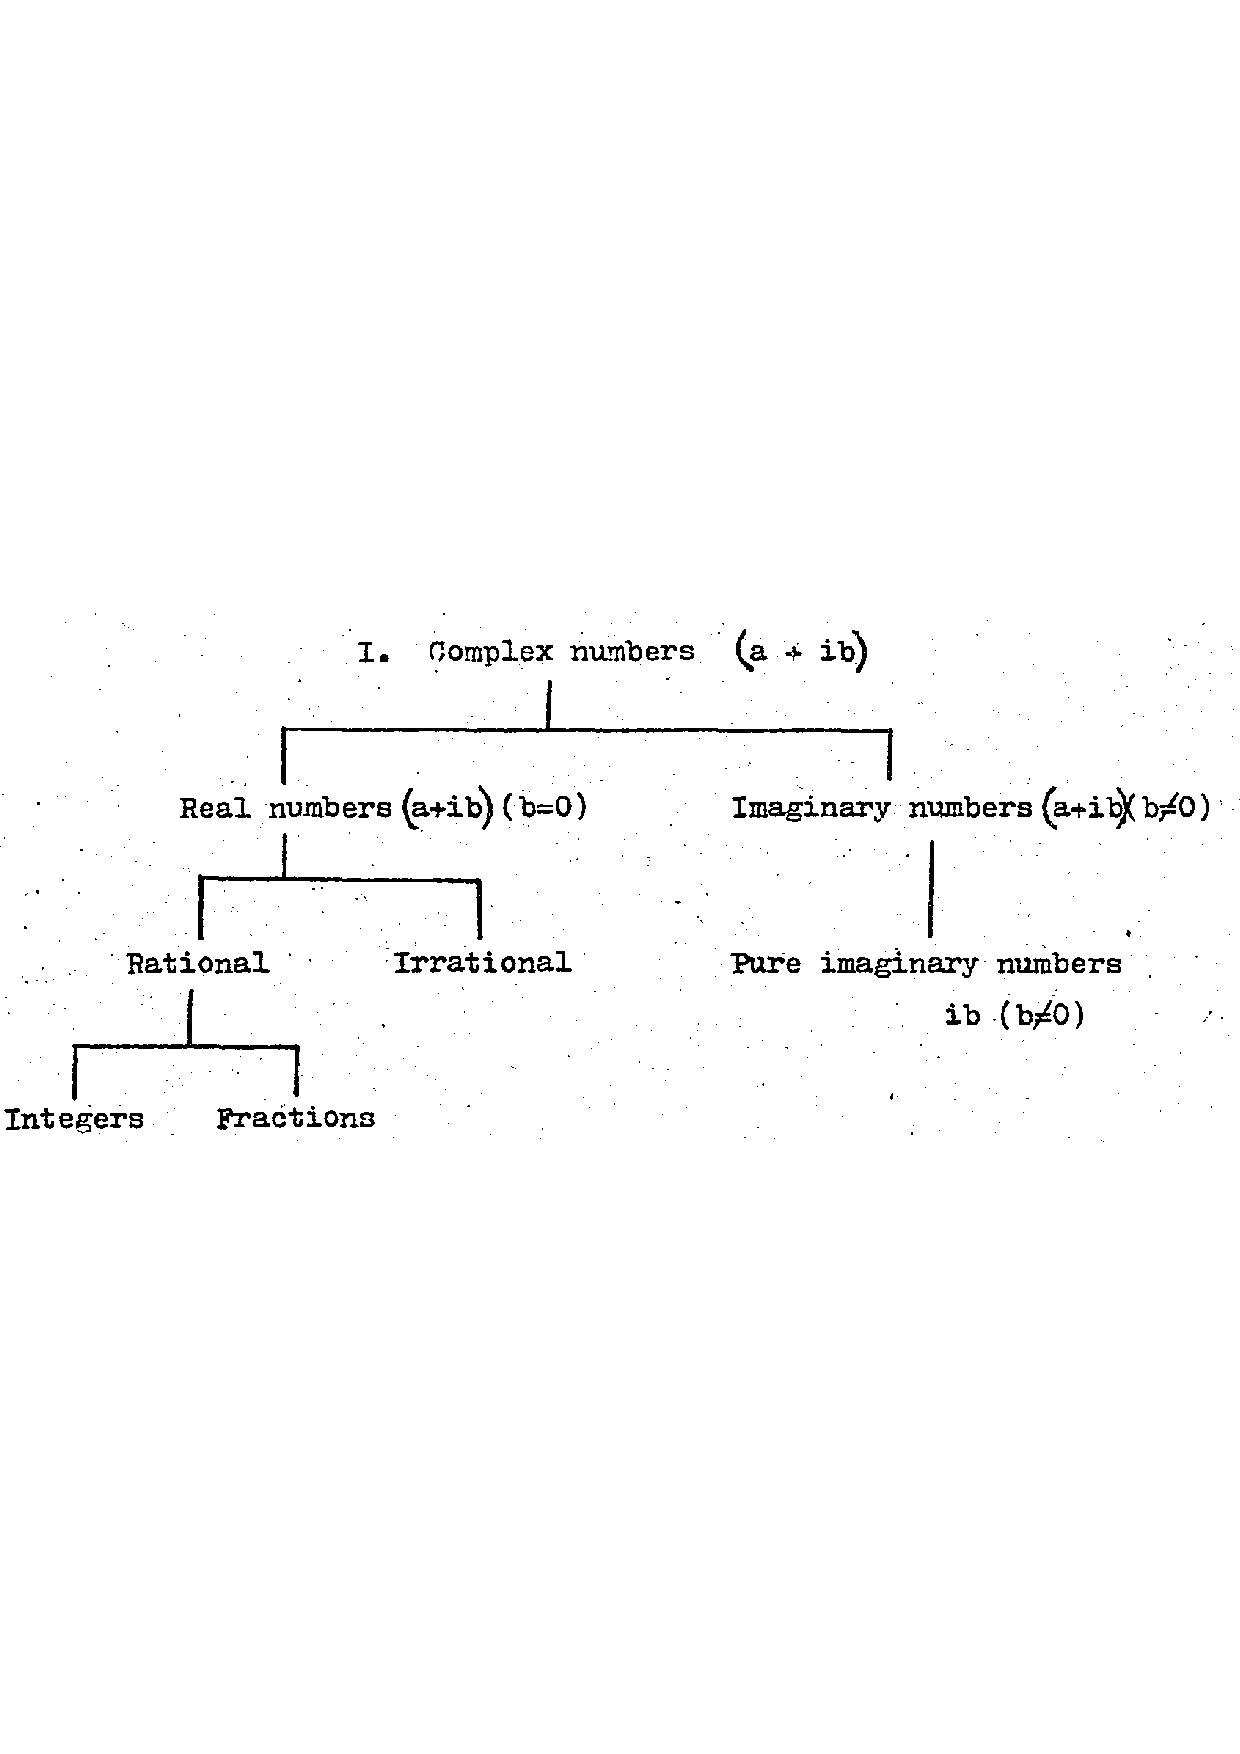
\includegraphics[width=0.9\textwidth]{images/SD-1-1p15A}
%	\caption{Classification of complex numbers}
%	\label{fig:classificationOfComplexNumbersA}
%\end{figure}

%\begin{center}
%\begin{tabular}{cc}
%\end{tabular}
%\end{center}

%\begin{exmp}
%\begin{hSolution}
%\end{hSolution}
%\end{exmp}

%\begin{hEnumerateAlpha}
%\end{hEnumerateAlpha}

%\begin{hEnumerateRoman}
%\end{hEnumerateRoman}

%$
%\begin{bmatrix}
%\end{bmatrix}
%$

%\frac{aaaa}{bbb}
%\frac{a_{n}}{b_{n}}
%\left( aaaa \right)
%\Longrightarrow

%\begin{multicols}{2}
%	bb
%\columnbreak
%	aa
%\end{multicols}
